\vspace{1in}
{\large
``The LHC accelerates \\
the protons and the lead, \\
and the things that it discovers \\
will rock you in the head."

\hfill - Katherine McAlpine, 2008}
\vspace{1in}

The results shown in this dissertation are obtained using the data collected by the ATLAS experiment at the LHC, the world's largest particle accelerator hosted by the European Organization for Nuclear Research (CERN). The LHC leads the energy frontier of particle physics enabling the exploration of $\mathcal{O}$(GeV) Heavy Neutral Leptons. ATLAS is one of the two multipurpose experiments at the LHC designed to probe a wide range of physics, spanning from precision measurements of the free parameters of the SM, to the direct searches of new BSM particles via unique signatures. Its large size along with its sophisticated yet versatile detector systems support the lifetime frontier making it a suitable detector to look for LLPs.

The LHC is described in \cref{sec:lhc} of this chapter. The ATLAS experiment is described in \cref{sec:atlas}, the reconstruction methods are explained in \cref{sec:reco}, and the dedicated reconstruction methods for the search of LLPs are described in \cref{sec:llp_reco}

\section{The Large Hadron Collider} \label{sec:lhc}

The Large Hadron Collider is a 27 kilometer proton or ion accelerator, designed to accelerate and collide protons at a center-of-mass energy ($\sqrt{s}$) of 13 TeV.

\begin{figure}
    \centering
    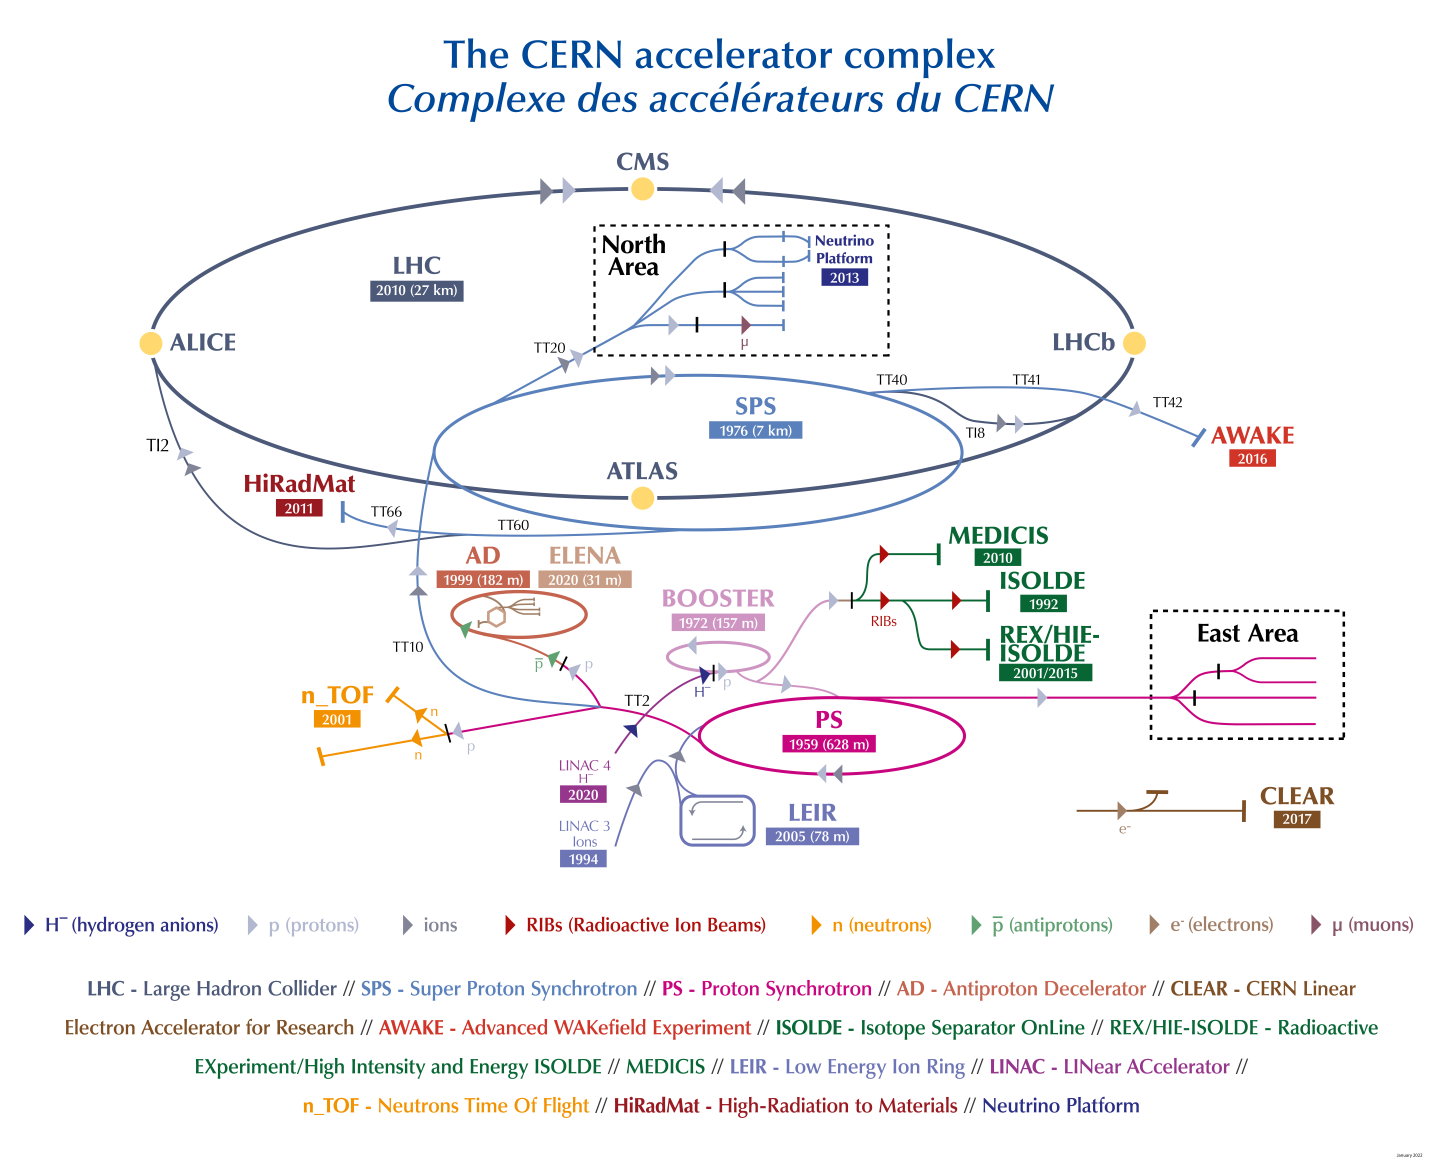
\includegraphics[width=0.5\linewidth]{figures/CCC-v2022.pdf}
    \caption{The CERN accelerator complex in 2022.\cite{Lopienska:2800984}}
    \label{fig:cern-acc-comp}
\end{figure}

\section{The ATLAS Experiment} \label{sec:atlas}

\section{Particle Reconstruction} \label{sec:reco}

\section{Dedicated Reconstruction for LLP Searches} \label{sec:llp_reco}